\documentclass{article}

\usepackage{graphicx}
\usepackage{amsmath}
\usepackage{amssymb}
\usepackage{siunitx}
\usepackage{hyperref} % for \url{}

% This stuff is for figures
\usepackage{float}
\DeclareGraphicsExtensions{.pdf, .png, .jpg}

\hypersetup{
    colorlinks=true,
    urlcolor=blue
}

\renewcommand{\c}[1]{\texttt{#1}}
%https://tex.stackexchange.com/questions/112932/today-month-as-text
\renewcommand{\today}{\ifnum\number\day<10 0\fi \number\day \space%
\ifcase \month \or January\or February\or March\or April\or May%
\or June\or July\or August\or September\or October\or November\or December\fi\space%
\number \year} 

\DeclareMathOperator{\norm}{\mathcal{N}}
\DeclareMathOperator{\unif}{unif}
\DeclareMathOperator{\expon}{expon}

\begin{document}

%\begin{flushright}
    \noindent
    Rodrigo Becerril Ferreyra\\
    E E 381 Section 12\\
    Lab 4\\
    \today
%\end{flushright}

\addcontentsline{toc}{section}{Introduction}
\section*{Introduction} The purpose to this lab is to explore
the Central Limit Theorem (CLT). Informally, the CLT states
that the sum of random variables \(X_1, X_2, \ldots, X_n\)
approaches a normal (Gaussian) distribution as \(n\to\infty\).
That is, for
\begin{gather*}
    Z = \sum_{i=1}^\infty X_i,\\
    P_Z(x) = \norm(Z = x; \mu, \sigma; \infty) = \frac1{\sigma\sqrt{2\pi}}\exp\left(-\frac{\left(x-\mu\right)^2}{2\sigma^2}\right)
\end{gather*} where \(P_Z(x)\) is the probability density
function (PDF) of \(Z\), \(\mu\) is the expected value of \(Z\),
and \(\sigma^2\) is the variance of \(Z\).

The notation I will use is the following: first is the
distribution name (e.g. \(\norm\)); next is the variable used to define
the distribution (e.g. \(X= x\)); next are the parameters
involved in the definition (e.g. \(\mu\) and \(\sigma\));
lastly, the number of samples generated in creating the
random variable (in other words, the length of the variable,
or the amount of discrete values associated with the variable).
This last value is necessary, because computers cannot
hold an infinite amount of data.

In this lab, we used both uniform distributions and
exponential distributions to test this theory. The PDF of the
(continuous) uniform distribution is given by the following
function:
\begin{equation*}
    \unif(X = x; a, b; \infty) =
    \begin{cases}
        \frac{1}{b-a} & \text{if } a \le x \le b\\
        0             & \text{otherwise}
    \end{cases}.
\end{equation*} The mean is given by \(\mu = (b+a)/2\) and
the variance given by \(\sigma^2 = (b-a)^2/12\).

The PDF of the exponential distribution
is given by
\begin{equation*}
    \expon(X = x; \lambda > 0; \infty) = \lambda e^{-\lambda x}
\end{equation*} where \(\mu = 1/\lambda\) and \(\sigma^2 = 1/\lambda^2\).
Note that in our lab, we used the parameter
\(\beta = 1/\lambda\); in this case,
\(\mu = \beta\) and \(\sigma^2 = \beta^2\).

\section{Problem 1}
\subsection{Question} In this problem, we were introduced
to the \c{numpy} commands to generate three random variables,
each representing one distribution.
We also calculated their expected value and standard
deviation, comparing them to the expected values.

For all PDF graphs, we generated \num{10000} values for each
random variable, then plotted it on a histogram. The blue
bars represent the generated values, and the red line
represents the theoretical PDF of that distribution.
Results are posted below. Note that Problem 1 took
about \SI{0.69}{s} in total to finish.

\subsection{Result 1} Below is the graph of the PDF of a
uniform distribution, and the table of experimental
and expected values. The distribution that was modeled
is \(\unif(X = x; 1, 4; \num{10000})\).

\begin{figure}[H]
    \centering
    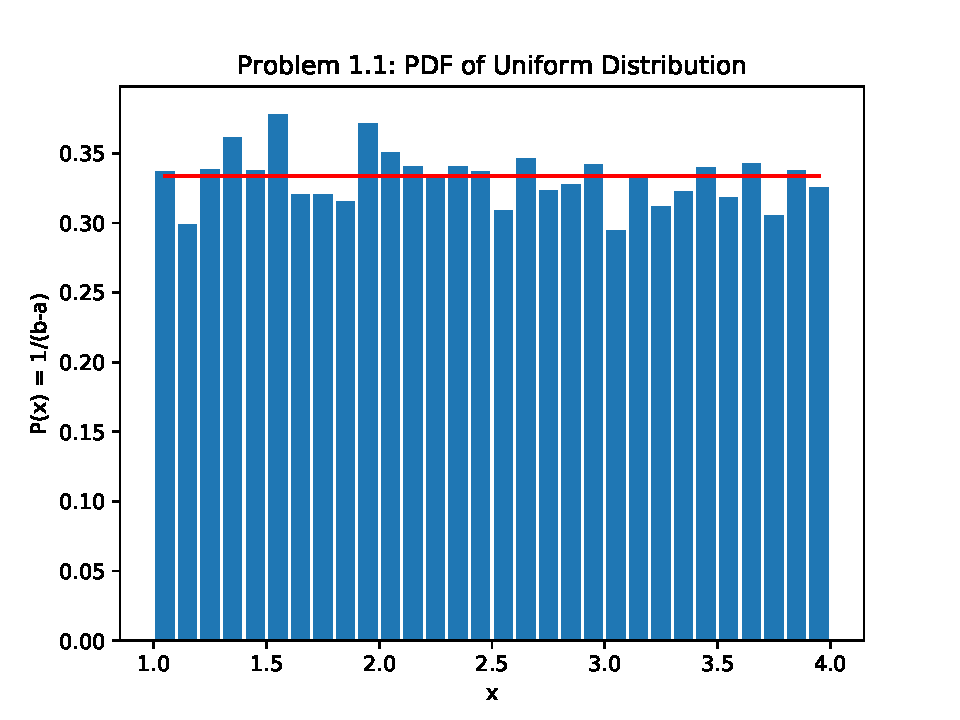
\includegraphics[width=\textwidth]{Images/Figure1}
    \begin{tabular}{|c|c|c|c|}
        \hline
        \multicolumn{4}{|c|}{Statistics for a Uniform Distribution}\\ \hline
        \multicolumn{2}{|c|}{Expected Value}                                                                                                      & \multicolumn{2}{c|}{Standard Deviation}\\ \hline
        \begin{tabular}[c]{@{}c@{}}Theoretical\\ Calculation\end{tabular} & \begin{tabular}[c]{@{}c@{}}Experimental\\ Measurement\end{tabular} & \begin{tabular}[c]{@{}c@{}}Theoretical\\ Calculation\end{tabular} & \begin{tabular}[c]{@{}c@{}}Experimental\\ Measurement\end{tabular} \\ \hline
        2.5 & 2.506 & \( \sqrt{3}/2 \) & 0.866 \\ \hline
    \end{tabular}
    \caption{Uniform Distribution Plot and Statistics}
    \label{P1:uniform}
\end{figure}

\subsection{Result 2} Below is the graph of the PDF of an
exponential distribution, and the table of experimental
and expected values. The distribution that was modeled
is \(\expon(X = x; 1/40; \num{10000})\).

\begin{figure}[H]
    \centering
    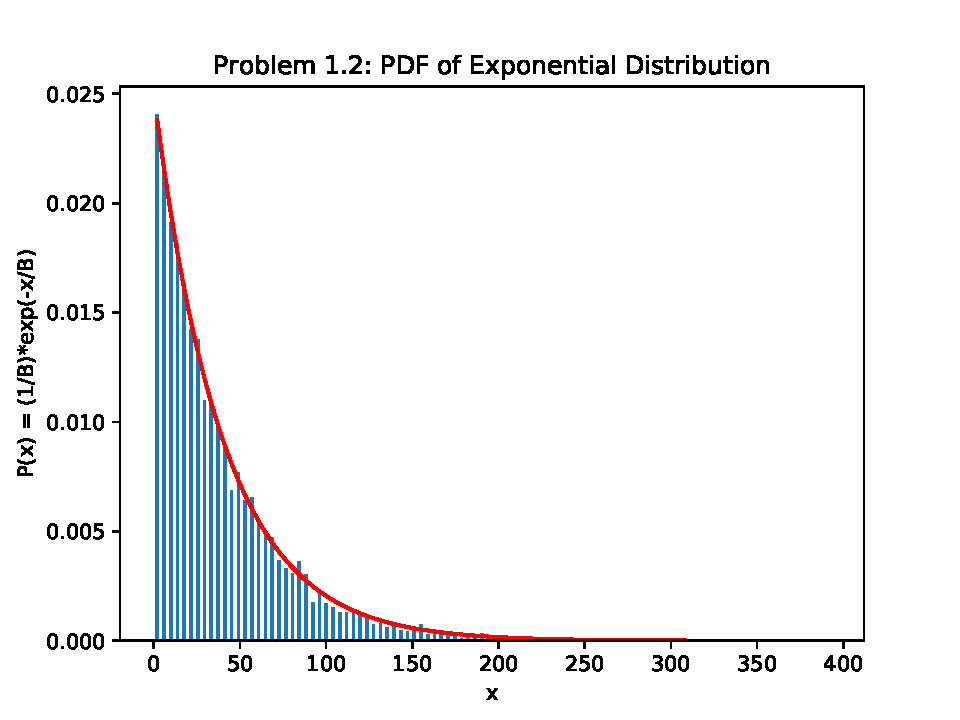
\includegraphics[width=\textwidth]{Images/Figure2}
    \begin{tabular}{|c|c|c|c|}
        \hline
        \multicolumn{4}{|c|}{Statistics for an Exponential Distribution} \\ \hline
        \multicolumn{2}{|c|}{Expected Value} & \multicolumn{2}{c|}{Standard Deviation} \\ \hline
        \begin{tabular}[c]{@{}c@{}}Theoretical\\ Calculation\end{tabular} & \begin{tabular}[c]{@{}c@{}}Experimental\\ Measurement\end{tabular} & \begin{tabular}[c]{@{}c@{}}Theoretical\\ Calculation\end{tabular} & \begin{tabular}[c]{@{}c@{}}Experimental\\ Measurement\end{tabular} \\ \hline
        40 & 39.91 & 40 & 40.00 \\ \hline
    \end{tabular}
    \caption{exponential Distribution Plot and Statistics}
    \label{P1:exponential}
\end{figure}

\subsection{Result 3} Below is the graph of the PDF of a
normal distribution, and the table of experimental
and expected values. The distribution that was modeled is
\(\norm(X = x; 2.5, 0.75; \num{10000})\).

\begin{figure}[H]
    \centering
    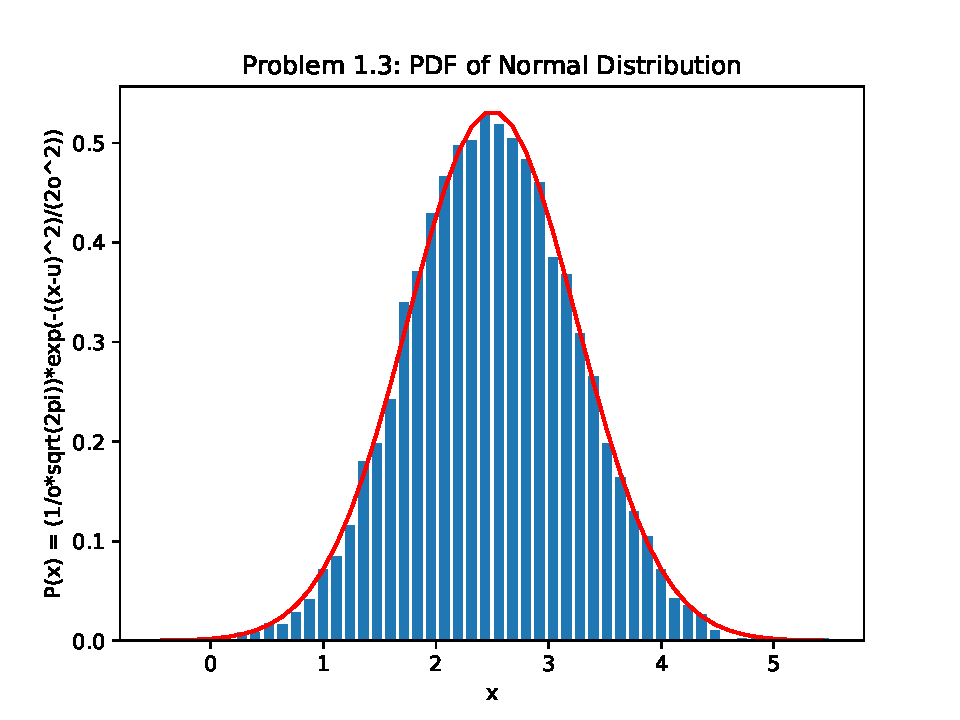
\includegraphics[width=\textwidth]{Images/Figure3}
    \begin{tabular}{|c|c|c|c|}
        \hline
        \multicolumn{4}{|c|}{Statistics for a Normal Distribution} \\ \hline
        \multicolumn{2}{|c|}{Expected Value} & \multicolumn{2}{c|}{Standard Deviation} \\ \hline
        \begin{tabular}[c]{@{}c@{}}Theoretical\\ Calculation\end{tabular} & \begin{tabular}[c]{@{}c@{}}Experimental\\ Measurement\end{tabular} & \begin{tabular}[c]{@{}c@{}}Theoretical\\ Calculation\end{tabular} & \begin{tabular}[c]{@{}c@{}}Experimental\\ Measurement\end{tabular} \\ \hline
        2.5 & 2.491 & 0.75 & 0.749 \\ \hline
    \end{tabular}
    \caption{Uniform Distribution Plot and Statistics}
    \label{P1:normal}
\end{figure}

\section{Problem 2}
\subsection{Question} In this problem, we are tasked with
setting up and witnessing the CLT in action. To do this,
we were tasked with creating four random variables
\begin{equation*}
    S_n = \sum_{i=1}^{\num{10000}} \unif(x; 1, 4; n)
\end{equation*} for \(n \in \{1, 5, 10, 15\}\).
In other words, \(S_n\) is the sum of \num{10000}
\(n\) uniformily-distributed random variables.
In this example, \(\unif(x; 1, 4; n)\) represents the thickness
of \(n\) books where each book can be anywhere within the
interval \(\left[ \SI{1}{cm}, \SI{4}{cm} \right)\).
The purpose of this
is to witness \(S_n\) converging to a normal distribution
as \(n\) gets larger. A table of the expected values and
standard deviations of \(S_n\) is given below
(note that these values are calculated values; the expected
values are displayed on the raw output, available at the
end of this lab report).
Note that
Problem 2 took about \SI{1.22}{s} to finish.

\begin{figure}[H]
    \centering
    \begin{tabular}{|c|c|c|}
        \hline
        \begin{tabular}[c]{@{}c@{}}Number of\\ books \(n\)\end{tabular} & \begin{tabular}[c]{@{}c@{}}Mean thickness of\\ a stack of \(n\) books\end{tabular} & \begin{tabular}[c]{@{}c@{}}Standard deviation of\\ a stack of \(n\) books\end{tabular} \\ \hline
        \(n=1\) & \( \mu_1 = 2.499 \) & \( \sigma_1 = 0.8633 \) \\ \hline
        \(n=5\) & \( \mu_5 = 12.53 \) & \( \sigma_5 = 1.935 \) \\ \hline
        \(n=10\) & \( \mu_{10} = 25.02 \) & \( \sigma_{10} = 2.750 \) \\ \hline
        \(n=15\) & \( \mu_{15} = 37.48 \) & \( \sigma_{15} = 3.372 \) \\ \hline
    \end{tabular}
    \caption{Mean and STD of \(S_n\).}
    \label{P2:table}
\end{figure}

\subsection{Result 1} The following is the PDF of \(S_1\).
Note that this plot does not follow the red line (a normal
distribution) at all. This is because \(n = 1\) and therefore
\(S_1\) follows a uniform distribution; there is nothing to
sum, because each uniform distribution only contains one value.
CLT only starts to
come out when \(n > 1\); even the example with \(n = 2\)
given in the lab manual is starting to look like a
normal distribution. This is because summing \num{10000}
uniform distributions is a lot.

\begin{figure}[H]
    \centering
    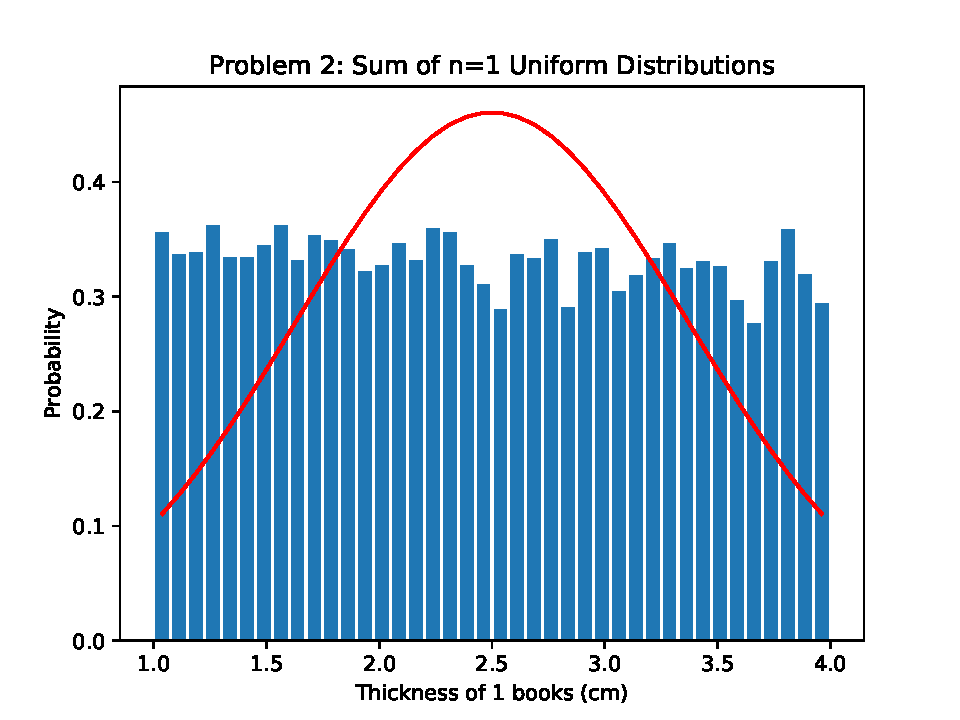
\includegraphics[width=\textwidth]{Images/Figure4}
    \caption{PDF of \(S_1\).}
    \label{P2:S1}
\end{figure}

\subsection{Result 2} The following is a PDF of \(S_5\).
This random variable, and the two that follow it, are more
reminiscent of a normally-distributed variable than \(S_1\).

\begin{figure}[H]
    \centering
    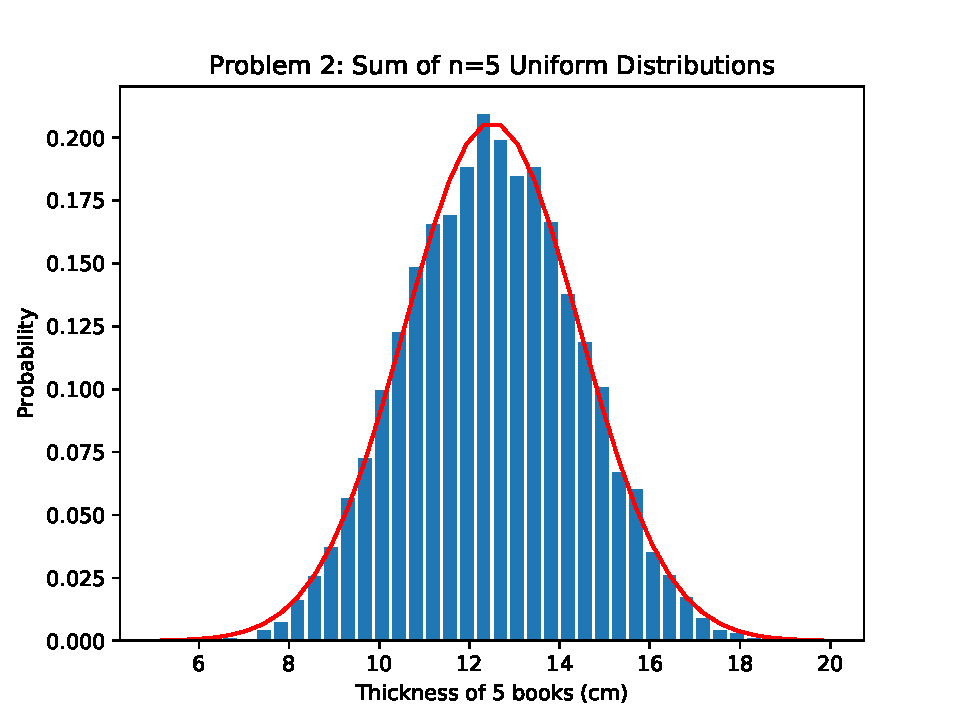
\includegraphics[width=\textwidth]{Images/Figure5}
    \caption{PDF of \(S_5\).}
    \label{P2:S5}
\end{figure}

\subsection{Result 3} The following is a PDF of \(S_{10}\).

\begin{figure}[H]
    \centering
    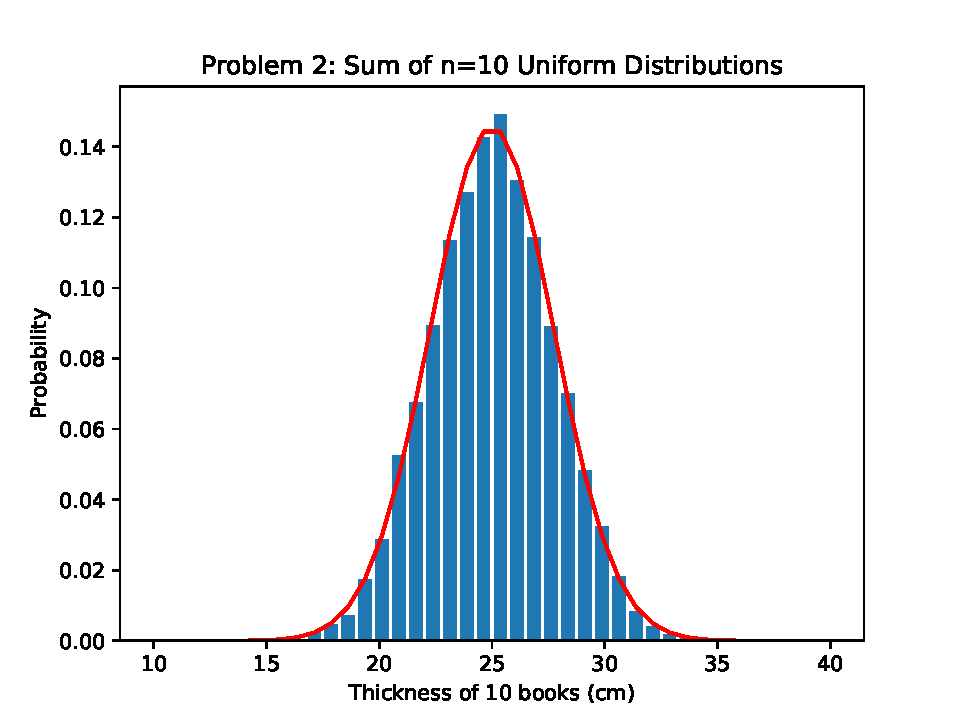
\includegraphics[width=\textwidth]{Images/Figure6}
    \caption{PDF of \(S_{10}\).}
    \label{P2:S10}
\end{figure}

\subsection{Result 4} The following is a PDF of \(S_{15}\).

\begin{figure}[H]
    \centering
    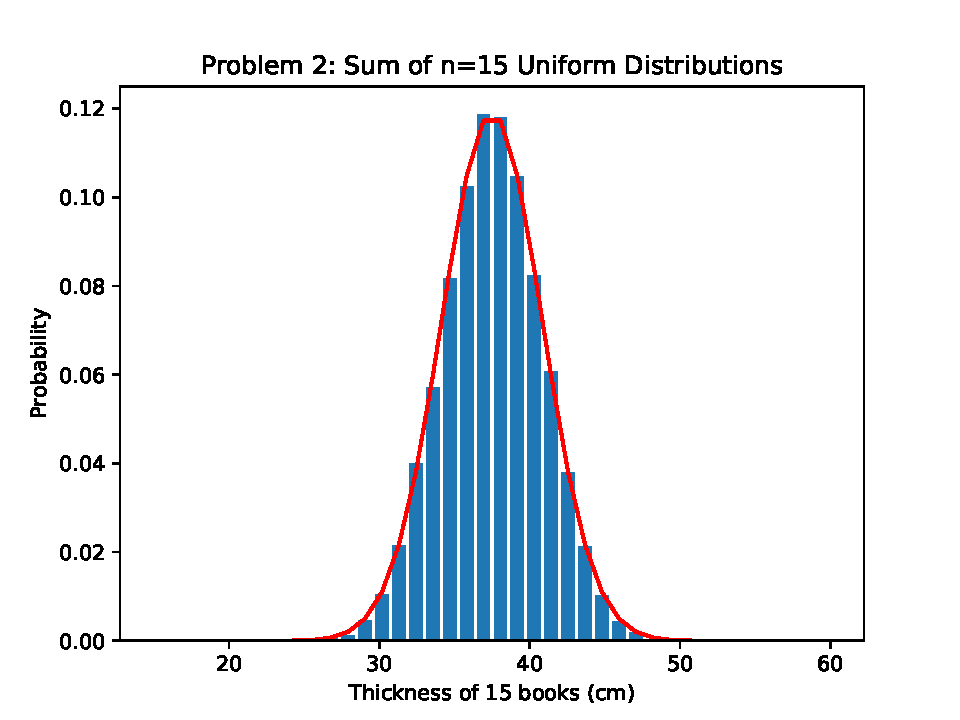
\includegraphics[width=\textwidth]{Images/Figure7}
    \caption{PDF of \(S_{15}\).}
    \label{P2:S15}
\end{figure}

\section{Problem 3}
\subsection{Question} This problem puts together all previous
ideas. In this scenario, 24 batteries come in a carton;
we are tasked with creating the random variable
\(C = \sum_{i=1}^{\num{10000}} \expon(x, 1/40, 24)\) and
figuring out the PDF and CDF of this random variable. The
two plots are as follows:

\begin{figure}[H]
    \centering
    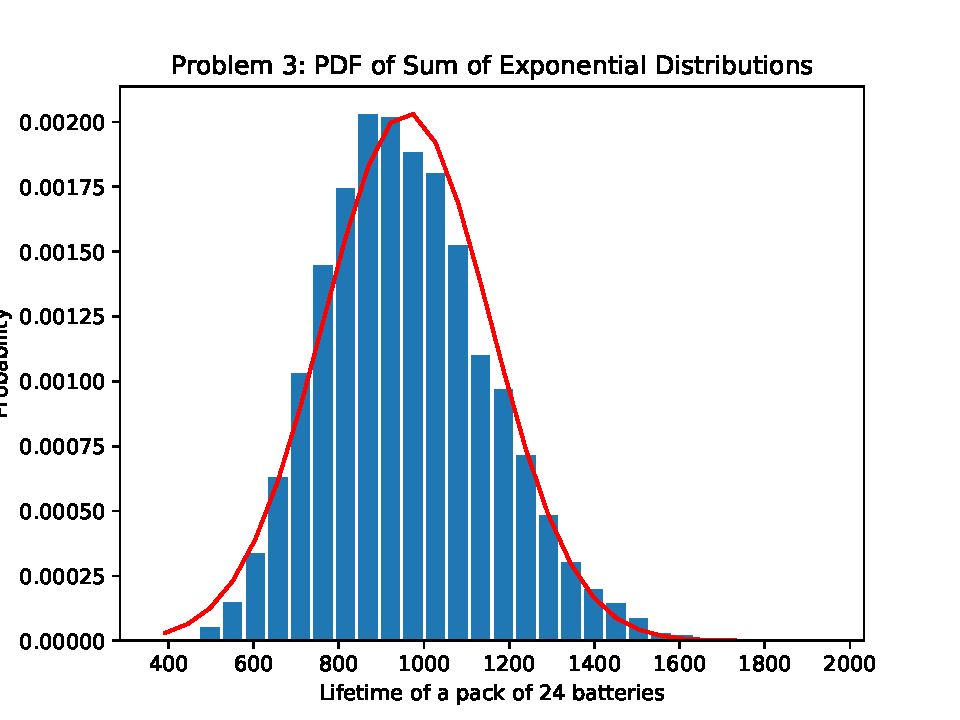
\includegraphics[width=\textwidth]{Images/Figure8}
    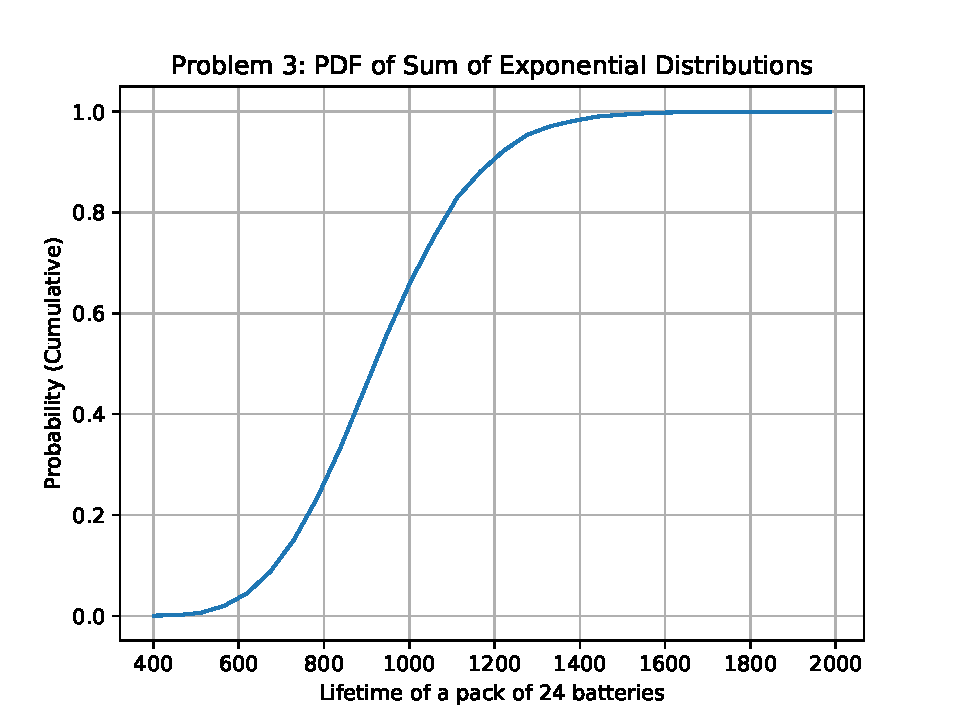
\includegraphics[width=\textwidth]{Images/Figure9}
    \caption{PDF and CDF of \(C\).}
    \label{P3}
\end{figure}

Again, this random variable is akin to a normally-distributed
random variable by CLT.

Using the plot of the CDF (because it is a vector graphic,
feel free to zoom in if viewing the PDF), we can determine the
following values:

{
\begin{tabular}{|l|r|}
    \hline
    \textbf{QUESTION} & \textbf{ANS.} \\ \hline
    1. Prob. that the carton will last longer than three years & \num{0.25} \\ \hline
    2. Prob. that the carton will last between 2.0 and 2.5 years & \num{0.275} \\ \hline
\end{tabular}
}

These values are obtained by the formulas \(1 - F(1095)\) and
\(F(912) - F(730)\), respectively; these are given in the
lab manual and are visual estimates only.

\section{Raw Output}
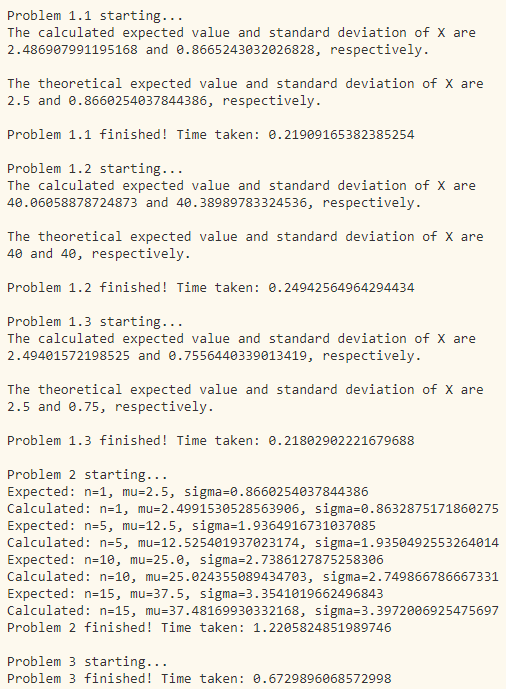
\includegraphics[width=\textwidth]{Images/output}

\end{document}
